\chapter{Methodology} \label{chap:3}

%-----------------------------------------------------------------------
%\section{Objective}
%-----------------------------------------------------------------------
This research investigated the behavior of additively manufactured cylindrical casings subjected to internal explosive loadings. Test samples were constructed using \gls{PBF} and filled with a controlled amount of explosives. The specimens were detonated inside indoor chambers while high speed cameras observed and recorded the detonation events. Fragmentation velocities and corresponding mechanical properties of the 15-5PH \gls{PBF}-printed stainless steel samples were derived from the captured images through \gls{DIC} analysis. Fragments formed during the detonation event were weighed to compare experimental results with classic fragment mass distribution models.

% %-----------------------------------------------------------------------
% \section{Theory}
% \label{sec:3_Theory}
% %-----------------------------------------------------------------------
% When an explosives-filled cylindrical casing is detonated, it's walls undergo rapid expansion before ultimately fracturing and
% The casing's material and mechanical properties determine its ability to elongate and withstand fracture during an explosion.

%-----------------------------------------------------------------------
\section{Specimen Design} \label{sec:3_specimen}
%-----------------------------------------------------------------------



Test samples were constructed via \gls{PBF} using 15-5PH stainless steel powder feedstock. \gls{PBF} was selected because of its ability to fabricate metal parts with mechanical properties suitable for high temperature environments. Additionally, 15-5PH stainless steel was chosen to synchronize this research with other ongoing \gls{DoD}-sponsored \gls{AM} projects, in addition to its favorable mechanical properties \cite{AFIT_Dempsey, EOS_StainlessSteel_M290}. The \gls{PBF} technique employed in this research was \gls{DLMS}.

\gls{DMLS} test specimens were manufactured by 3Diligent in El Segundo, California and by i3D MFG, located in Bend, Oregon.
3Diligent samples were constructed using an EOS \gls{DMLS} system (exact model considered proprietary information) and i3D MFG specimens were fabricated using EOS's EOSINT M 280 system. Both companies used EOS's StainlessSteel PH1 feedstock, a 15-5PH stainless steel powder featuring the chemical composition given below in \cref{tab:3Diligent_Chem_Comp}:

% Tab - 3Diligent Material Composition
\FloatBarrier
\begin{table}[h]
  \centering
  \caption{Chemical composition of 15-5 PH Stainless Steel feedstock used by 3Diligent and i3D MFG for \gls{DMLS} cylinder printing  \cite{EOS_StainlessSteel_M290}}
    \begin{tabular}{lc}
    \multicolumn{2}{c}{\textbf{\large EOS StainlessSteel PH1}} \\
    \midrule
    \multicolumn{1}{c}{\textbf{Element}} & \textbf{Percentage (weight)} \\
    \midrule
    Iron (Fe) & (balance) \\
    Chrormium (Cr) & 14.0 - 15.5 \\
    Nickel (Ni) & 3.5 - 5.5  \\
    Copper (Cu) & 2.5 - 4.5 \\
    Manganese (Mn) & 1.00 \\
    Silicon (Si) & 1.00 \\
    Carbon (C) & 0.07 \\
    Molybdenum (Mo) & 0.5 \\
    Niobium (Nb) & 0.15 - 0.45 \\
    \bottomrule
    \end{tabular}%
    \label{tab:3Diligent_Chem_Comp}%
\end{table}
\FloatBarrier
Following construction and a post-processing precipitation hardening treatment of 480\degree C for 4 hours, room temperature tensile testing of EOS's StainlessSteel PH1 in accordance with ISO 6892:1998(E) Annex C yields the following mechanical properties:

% Table generated by Excel2LaTeX from sheet '3Diligent'
\begin{table}[htbp]
  \centering
  \caption{3Diligent's 15-5 PH stainless steel mechanical properties \cite{EOS_StainlessSteel_M290}}
    \begin{tabular}{lc}
    \multicolumn{2}{c}{\textbf{\large EOS StainlessSteel PH1}} \\ 
    \midrule
    %
    \multicolumn{2}{l}{\textbf{Ultimate Tensile Strength (MPa)}} \\
    Longitudinal & 1440 $\pm$ 100 \\
    Transverse  & 1450 $\pm$ 100 \\[1 ex]
    %
    \multicolumn{2}{l}{\textbf{Yield Strength (MPa)}} \\
    Longitudinal & 1350 $\pm$ 100 \\
    Transverse & 1300 $\pm$ 100 \\[1 ex]
    %
    \multicolumn{2}{l}{\textbf{Elongation at Failure (\%)}} \\
    %\midrule
    Longitudinal & 13 $\pm$ 3 \\
    Transverse  & 15 $\pm$ 3 \\
    \bottomrule
    \end{tabular}%
  \label{tab:addlabel}%
\end{table}%
Components produced using EOS's StainlessSteel PH1 powder and M 290 printer have a density of approximately 7.7 g/cm$^{3}$ (compared to a $\sim$7.8 g/cm$^{3}$ density exhibited by conventional 15-5 PH stainless steel H900 \cite{AKSteel_Conventional_SS}) and a 20 $\mu$m layer thickness \cite{EOS_StainlessSteel_M290}.

%%%%%%% i3D MFG Section %%%%%%%%
\gls{DMLS}-printed casings were constructed by Oregon-based i3D MFG using EOS's StainlessSteel PH1 powder (\label{tab:3Diligent_Chem_Comp}) and M 290 printer



...The material composition of 15-5 PH Stainless Steel used by i3D MFG is shown in   




%Thirty specimens were fabricated for each of the three models, totaling 90 test samples for the experiment. 
%In total, x samples were detonated...


%%%%%%%%%%%%%%%%%%%%%%%%%%%%%%%%%%%%
\subsection{Specimen Dimensions} \label{sec:3_specimen_dimensions}
%%%%%%%%%%%%%%%%%%%%%%%%%%%%%%%%%%%%

Due to budget and time constraints, small-scale test samples ($C <$ 1 g) were used to maximize the amount of data collected during the allocated test window. Researchers at \gls{SNL} discovered fragmentation properties of metallic casings undergoing explosive loading remain largely unchanged when scaled down appropriately (private communication). This significantly reduces experimental preparation and completion times, allowing for more detonation events in a given time frame. 

In order to capture the effects of varying the explosive to casing mass ratio $C/M$, three different casing \gls{CAD} models were built, each having a unique outer diameter $d_{outer}$. By holding all other dimensions constant, this produced a variation in casing mass $M$, and thus different $C/M$ values, producing the experiment's control variable. An example \gls{CAD} model is shown in \Cref{fig:3_Casing_CAD_model}, and \Cref{fig:3_Casing_dimensions} compares the three models' dimensions. Both manufacturers received the same \gls{CAD} models to minimize variation in the test specimens.

%Fig - An example showing one of the CAD models
\begin{figure}[H]
	\centering
 \fbox{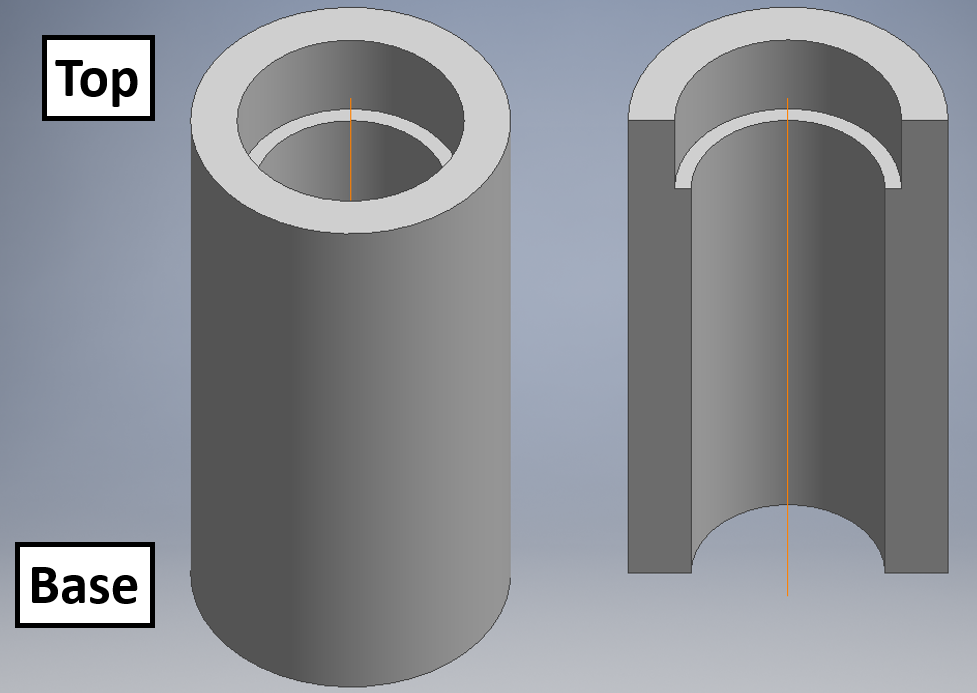
\includegraphics[width=0.6\linewidth]{Ch3/Figures/Example_CAD_Model.PNG}}
    \caption{Example casing \gls{CAD} model}
	\label{fig:3_Casing_CAD_model}
\end{figure}
%
%
\begin{figure}[H]
	\centering
 \fbox{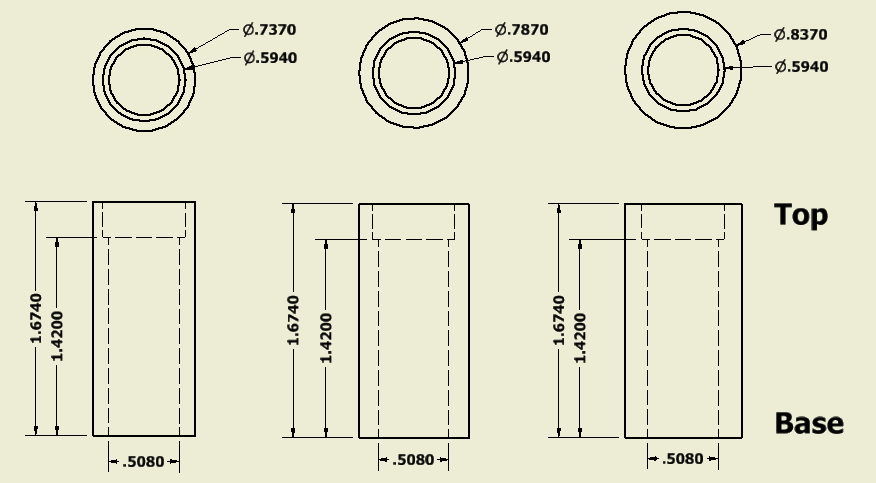
\includegraphics[width=1.0\linewidth]{Ch3/Figures/CAD_Model_Comparison.PNG}}
    \caption{Dimensions of the three test specimens used in this research (all dimension values in cm)}
	\label{fig:3_Casing_dimensions}
\end{figure}
%

%%%%%%%%%%%%%%%%%%%%%%%%%%%%%%%%%%%%
\subsection{RP-80 Detonator} \label{sec:3_RP80}
%%%%%%%%%%%%%%%%%%%%%%%%%%%%%%%%%%%%
Detonators are traditionally used to initiate an explosion of a larger mass of explosives; however, \gls{SNL} converted Teledyne RISI's RP-80 exploding bridgewire detonator (\Cref{fig:3_RP-80_Layout}) into a ``surrogate" explosive device for sub-scale fragmentation testing. This is accomplished by replacing the RP-80's explosive train casing with the test specimen, creating a standalone explosive with the RP-80's internal 0.203 g of explosive filling. %Reword? 

%insert two figures, overall rp-80, and outer casing
%by fitting sleeves around the detonator's internal explosives.

%Fig - RP-80 design with cross section showing the explosive train's internal components
\begin{figure}[H]
	\centering
 \fbox{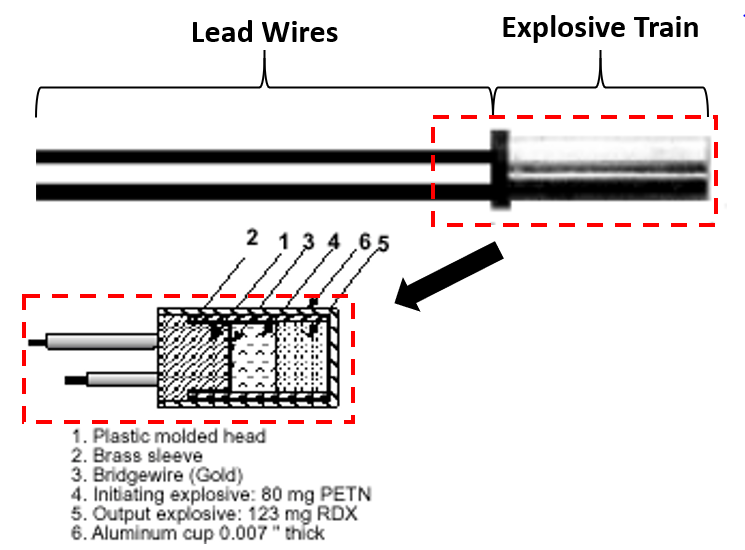
\includegraphics[width=0.6\linewidth]{Ch3/Figures/RP-80_Layout.PNG}}
    \caption{RP-80 detonator design, with a cross section adapted from Teledyne RISI's website illustration\cite{TeledyneRP-80}}
	\label{fig:3_RP-80_Layout}
\end{figure}
%
%Furthermore, by replacing the manufacturer's original outer sleeve with the test cylinder 
%commercial detonators are provide sufficient explosive filling (Private communication).    
%employed in this research, using an RP-80 detonator as the explosive filling.


%%%%%%%%%%%%%%%%%%%%%%%%%%%%%%%%%%%%
\subsection{Sample Manufacturing \& Preparation} \label{sec:3_Sample_Manufacturing}
%%%%%%%%%%%%%%%%%%%%%%%%%%%%%%%%%%%%
\begin{spacing}{1}
\noindent
\textbf{\textit{(rough draft note: Additional manufacturing details and images will be added once test specimens are constructed )}}
\end{spacing}
\vspace{1cm}

Test sample \gls{CAD} models were designed in Autodesk Inventor and then converted into STEP files for \gls{SLM} machine compatibility. These files were provided to I3DMFG...

After manufacturing was complete, 0.200 cm of length was removed from cylinders' bases via Wire \gls{EDM} to compensate for build plate effects generated during \gls{DMLS}, yielding an overall length of 1.474 cm for all test specimens. 

Test samples were filled with ...g of \gls{PETN} by explosives experts from \gls{SNL} and bored to remove any variations resulting from \gls{DMLS} processing.

Furthermore, \gls{AM}-printed 15-5PH stainless steel has exhibited tensile properties comparable to wrought and cast metals in previous research, further increasing its... 

%Paragraph on how Dan uses RP-80 for subscale testing of material fragmentation behavior, need to source this

%The RP-80 is an electronic bridgewire detonator used

%\ref{method_RP-80}
%Due to its design, the RP-80 detonator samples were limited to a L/D ratio of xx or lower. Consequently,....end effects 
%The sleeve's inner diameter was held constant to...
%By varying outer diameter and length within allowable limits, sleeves were constructed...  

%-----------------------------------------------------------------------
\section{Data Collection System} \label{sec:3_specimen}
%-----------------------------------------------------------------------

Two Shimadzu HPV-X2 high speed cameras were used to capture the detonation events using a [number] \gls{fps} frame rate..... This stereo camera configuration enables three-dimensional material displacement and deformation measurements during the subsequent \gls{DIC} analysis (\Cref{sec:3_digital_image_correlation}).  The cameras were mounted on sliding brackets .... 

For each test event, 128 images were recorded and stored on the cameras' onboard memory system, using a signal from the... to trigger the recording.


Two laser light sources, Cavitar's CAVILUX Smart and Specialised Imaging's SI-LUX640, were used to illuminate the detonation events. These systems were configured to emit 640 nm wavelength pulsed laser light and synchronized with the selected camera frame rate. To minimize the amount of background and detonation-generated light reaching the lenses and infiltrating the recorded images, both cameras were fitted with optical filters, restricting allowable light transmission to 640 $\pm$ 10 nm wavelengths.  


%In order to optimize high speed camera.... while.... minimize the influence of unwanted light sources,


%-----------------------------------------------------------------------
\section{Experimental Procedure} \label{sec:experimental_procedure}
%---------------------------------------------------
To maximize the amount and breadth of data collected


%%%%%%%%%%%%%%%%%%%%%%%%%%%%%%%%%%%%
\subsection{Overall Field of View } \label{sec:3_specimen_dimensions}
%%%%%%%%%%%%%%%%%%%%%%%%%%%%%%%%%%%%
The first three detonations focused on characterizing overall cylinder behavior 


%First, a large field of view test was performed to determine the optimal size window for \gls{DIC} data collection 



Test samples were detonated inside \gls{SNL}'s [specific chamber name] indoor explosives chambers. High speed cameras were positioned outside of the chambers....Following test completion, the captured images were exported to the computer system for follow-on \gls{DIC} analysis.
%-----------------------------------------------------------------------
\section{\glsentryfull{DIC} Analysis} \label{sec:3_digital_image_correlation}
%-----------------------------------------------------------------------
\begin{spacing}{1}
\noindent
\textbf{\textit{(rough draft note: This section will be completed after performing the experimental testing and \gls{DIC} analysis)}}
\end{spacing}
\vspace{1cm}


\gls{DIC} analysis was performed using \gls{SNL}'s DICe software package....

%and \gls{SNL}'s DICe software package was used for \gls{DIC} analysis. \cite{ReuDICapplication}

%-----------------------------------------------------------------------
\section{Fragment Mass Measurements}
\label{sec:3_digital_image_correlation}
%-----------------------------------------------------------------------
\begin{spacing}{1}
\noindent
\textbf{\textit{(rough draft note: This section will be completed after performing experimental mass measurements)}}
\end{spacing}
\vspace{1cm}


Fragment masses were measured using....This scale has a tolerance of...After all measured values were recorded,....

%-----------------------------------------------------------------------
\section{Summary} \label{sec:3_summary}
%-----------------------------------------------------------------------
Chapter 3 details the experimental approach used to study and characterize fragmentation properties of explosives-filled additively manufactured cylinders. Test samples designed in Autodesk Inventor software were fabricated via \gls{DMLS}. After filling the specimens with explosives, detonations were performed inside indoor blast chambers with high speed cameras monitoring casing expansion and fragmentation. After data collection was concluded, fragmentation properties were computed using \gls{DIC} analysis and fragment mass measurements.


